\graphicspath{{Figs/montecarlo/}}

%
% To start the document, use
%  \chapter{...}
% For lover level, sections use
%  \section{...}
%  \subsection{...}
%
\chapter{Reversed Monte Carlo Scattering: ARTS-MC}
 \label{sec:montecarlo}


%
% Document history, format:
%  \starthistory
 %    date1 & text .... \\
%    date2 & text .... \\
%    ....
%  \stophistory
%
\starthistory
  120410 & Moved from user guide to theory document.\\
  300504 & Created and written by Cory Davis.\\
\stophistory


%
% Symbol table, format:
%  \startsymbols
%    ... & \verb|...| & text ... \\
%    ... & \verb|...| & text ... \\
%    ....
%  \stopsymbols
%
%

%
% Introduction
%




\section{Introduction}
 \label{sec:montecarlo:intro}

%\subsection{Briefly what is Monte Carlo and why}
The ARTS Monte Carlo scattering module (ARTS-MC) offers an efficient method for
polarized radiative transfer calculations in arbitrarily complex 3D
cloudy cases.  The algorithm solves the integral form of the Vector Radiative Transfer Equation (VRTE), by applying Monte Carlo integration with
importance sampling (MCI) (e.g. \citep{numerical_recipes_C:97}).
As described in \citep{battaglia07:_microw_jqsrt}, when compared to other techniques for solving the VRTE in 3D domains the ARTS-MC
algorithm has the following advantages:
\begin{itemize}
\item All computational effort is dedicated to calculating the Stokes
 vector at the location of interest and in the direction of
 interest. This is in contrast to forward Monte Carlo and discrete ordinate methods
 where the whole radiation field is calculated.
\item CPU and memory cost scale more slowly than discrete ordinate methods with
 grid size, so that large or detailed 3D scenarios are not a problem. 
\item Only parts of the atmosphere that
 significantly contribute to the observed radiance are considered in the
 computation. Where the medium is optically thick, only the parts of the atmosphere closest
 to the sensor are visited by the algorithm.  This contrasts with DOM
 methods, where the whole radiation field is
 computed, and in particular with forward Monte Carlo methods, where added optical thickness
 further restricts the number of photons reaching the sensor.
\end{itemize}

%\subsection{Introduce published paper(s?) and outline the difference of this document}
The Monte Carlo integration of the VRTE is over infinite dimensions, where for each scattering order there is a
dimension representing: path-lengths, the choice between emission and scattering, and the choice between reflection or emission at the earth's surface.  In practice the integrand is always calculated for
a finite scattering order, as the dimensionality of the integral is
truncated by photon emission or the boundary of the domain.  
Thus, the algorithm can be pictured as tracing a large number of photons backwards from sensor, in
randomly selected multiply scattered propagation paths to either their
point of emission, or entry into the scattering
domain.  This physical
picture is identical to the Backward-Forward Monte Carlo algorithm
described by \citep{liuetal:96}. However, BFMC did not account for
dichroism, which is correctly accounted for in ARTS-MC by importance sampling. 

The description of reversed Monte Carlo as tracing photon paths backwards from the sensor gives a useful first-order physical picture for understanding the algorithm, but can lead to difficulty understanding the veracity of the method with regard to polarization.  These difficulties are not apparent in the scalar radiative transfer case\footnote{Although this physical picture of reversed Monte Carlo radiative transfer in the scalar case makes intuitive sense, the mathematical demonstration of how this method solves the Schwarzchild equation is often neglected}. Specifically, questions I have been asked that highlight the difficulty have included:
\begin{itemize}
\item how can you sample a single reversed pathlength when the medium is dichroic? (i.e. different extinction for the different polarized components)
\item when reverse tracing, how can you decide on a scattering or emission event when the single scattering albedo depends on the polarization state of the incoming photon?
\item How can you sample a single reverse scattered (i.e. incoming) direction when the scattered polarization state depends on the polarization state of the incoming photon?
\end{itemize}
The answer in each case is to forget the physical picture, focus on the mathematical solution to the VRTE, and realise that MCI permits some freedom in the choice of probability density functions (PDFs), provided the sampled integrand is properly weighted.   In the model presented here we choose PDFs that aim to minimise the variance in the 1st element of the Stokes vector.  This issue does not arise in the scalar case because it is possibile to perfectly sample the phase function to choose new incoming directions, and perfectly sample the transmission function to choose pathlengths, so no weighting terms appear. With the above difficulties in mind, in comparison with \citep{davisetal:04}, the algorithm description presented here is more in the context of MCI and with less reference to reversed traced photons.  What were referred to as photons in \citep{davisetal:04} we now call Stokes Vector Evaluations (SVE).

The current implementation of the algorithm differs slightly from the description in \citep{davisetal:04}; changes include:
\begin{itemize}
\item the initial line of sight is no longer treated differently than the scattered paths 
\item the algorithm is no longer confined to the `cloudbox', 
\item MCI is now used for convolving the simulated Stokes vector with a 2D antenna response (\citep{davisetal:04} discusses only pencil beam calculations)
\item MCI is now used to treat emission or reflection from the earth's surface.
\end{itemize}
These changes make the algorithm simpler and more general.


%%%%%%%%%%%%%%%%%%%%%%%%%%%%%%%%%%%%%%%%%%%%%%%%%%%%%%%%%% 
\section{Model}
 \label{sec:montecarlo:model}
The radiative transfer model solves the vector
radiative transfer equation (VRTE):
\begin{eqnarray}
\frac{d\mathbf{I(n)}}{ds}=-\mathbf{K(n)I(n)} +
\mathbf{K_a(n)}I_b(T) +\nonumber\\
\int_{4\pi}\mathbf{Z(n,n')I(n')}d\mathbf{n'}
\label{vrte}
\end{eqnarray}
where $\mathbf{I}$ is the 4 element column vector of radiances
$\mathbf{I}=\left[I,Q,U,V\right]^T$ with units
(Wm$^{-2}\mu$m$^{-1}$sr$^{-1}$). This will be referred to as the
Stokes vector, although normally the Stokes vector is expressed in
units of intensity.  $s$ is distance along direction $\mathbf{n}$ and
$I_b$ is the Planck radiance. $\mathbf{K(n)}$, $\mathbf{K_a(n)}$,
and $\mathbf{Z(n,n')}$ are the bulk extinction matrix, absorption
coefficient vector and phase matrix of the medium respectively.  For
 brevity these have been expressed as bulk optical
properties, where individual single scattering properties have been
multiplied by particle number density and averaged over all
orientations and particle types. The argument $\mathbf{n}$ has been
retained to signify that in general these properties depend on the
direction of propagation. 

To apply Monte Carlo integration to the problem, the VRTE needs to be expressed in integral form. (e.g. \cite{hochstadt:64})
\begin{eqnarray}
\lefteqn{\mathbf{I(n,s_0)}=\mathbf{O(u_0,s_0)I(n,u_0)}+}\nonumber\\
& \int_{u_0}^{s_0}\mathbf{O(s',s_0)}\left(\mathbf{K_a(n)}I_b(T) +\int_{4\pi}\mathbf{Z(n,n')}\mathbf{I(n')}d\mathbf{n'}\right)ds'\nonumber
\end{eqnarray}
\begin{equation}
\label{intVRTE}
\end{equation}
, where $\mathbf{O(s',s)}$ is the evolution operator defined by
\cite{landi:85}. $\mathbf{u_0}$ is the point where the line of sight intersects
the far boundary of the scattering domain, and $\mathbf{s_0}$ is the
exit point where the outgoing Stokes vector is calculated.

\subsection{Integration over the antenna response function}

If we consider a scalar antenna response function,
$\psi=\psi(\theta,\phi)=\psi(\mathbf{n})$, where $\psi(\mathbf{n})$ is
normalised such that $\int_{4\pi}\psi(\mathbf{n})dn=1$, then the
observed Stokes vector $\mathbf{I_{ant.}(n,s_0)}$ will be

\begin{equation}
\mathbf{I_\psi(n,s_0)}=\int_{4\pi}\psi(\mathbf{n'})\mathbf{I(n',s_0)}d\mathbf{n'}
\label{antInt}
\end{equation}

If we apply Monte Carlo integration with importance sampling to
Eq. \ref{antInt} and sample $\mathbf{n'}$ according to a probability
density function (PDF) equal to $\psi(\mathbf{n'})$, an unbiased
estimate of Eq. \ref{antInt} is given by (e.g. \cite{press:92})

\begin{eqnarray}
\mathbf{I_\psi(n,s_0)}&=&\int_{4\pi}\mathbf{I(n',s_0)}\psi(\mathbf{n'})d\mathbf{n'}\\
&\approx&\langle \mathbf{I(n',s_0)} \rangle_\psi
\label{antIntMC}
\end{eqnarray}
, where the angled brackets indicate the arithmetic mean, and the $\psi$ subscript indicates the sampled PDF.  Eq. \ref{antIntMC} has an estimated error for each Stokes index, $j$,  of
\begin{equation}
\delta I_j=\sqrt{\frac{\langle I_j^2\rangle-\langle I_j\rangle^2}{N}}.
\label{error}
\end{equation}

\subsection{The path integral}
\label{sec:path_integral}
We now require a Monte Carlo estimate of the integrand in
Eq. \ref{antIntMC}, which is given by Eq. \ref{intVRTE}.  First, we
re-express \ref{intVRTE} as a single integral, for simplicity dropping
the prime on $\mathbf{n'}$,

\begin{equation}
\mathbf{I(n,s_0)}=\int^{s_0}_\infty\left\{\begin{array}{rl}
\mathbf{O(s',s_0)}\left(\mathbf{K_a(n)}I_b(T)
+\int_{4\pi}\mathbf{Z(n,n')}\mathbf{I(n')}d\mathbf{n'}\right) & s'< s'_{boundary} \\
\frac{\mathbf{O(u_0,s_0)I(n,u_0)}g}{\int^\infty_{u_0}gds} & s'\ge s'_{boundary}
\end{array}ds'\right.
\label{inorouteq}
\end{equation}
, where $g$ is the PDF we will eventually use to sample pathlength,
$\Delta s$. $s'_{boundary}$ represents the pathlength corresponding to
the boundary of the domain opposite the line of sight.
The integrand Eq. \ref{inorouteq} is a piecewise function of the
path distance, where path distances corresponding to positions outside
the modelled domain give a boundary radiance attenuated by the evolution
operator over the length of the path within the model domain, and path
distances corresponding to points within the modelled atmosphere give
a sum of emission and scattering attenuated by the evolution operator
over the distance between the point and the atmosphere exit. 
The reader
could easily verify that evaluating Eq. \ref{inorouteq} is equivalent
Eq. \ref{intVRTE}. 

The aim in importance sampling is to choose probability density functions
(PDFs) for the independent variables that are
as close as possible to being proportional to the integrand
\cite{liu:01}. This concentrates computational effort on regions where
the integrand is most significant and also reduces the variance in the Stokes Vector evalations (SVE), thus reducing
the number of SVEs and hence CPU time required to give a
prescribed accuracy.  Eq. \ref{intVRTE} suggests that the PDF for
sampling path length, where path length is the distance traced backwards
from the sensor, $\Delta s=\left|\mathbf{s}-\mathbf{s'}\right|$, should be proportional in some way to the evolution
operator $\mathbf{O(s',s)}$. 

In general there is no closed form expression for $\mathbf{O(s',s)}$.
However, in cases where the extinction matrix is constant along a
propagation path
\begin{equation}
\mathbf{O(s',s)}=\exp\left(-\mathbf{K}\Delta s\right)
\label{OconstK}
\end{equation}
In ARTS a propagation path consists of a set of coordinates
indicating where the path intersects with grid surfaces.  If the
extinction matrix in the path segment between two such points is
considered constant, $\mathbf{K}=(\mathbf{K_j}+\mathbf{K_{j+1}})/2$,
the evolution operator between two arbitrary points $\mathbf{s_0}$ and
$\mathbf{s}_N$ is
\begin{eqnarray}
\mathbf{O}(\mathbf{s}_0,\mathbf{s}_N) =
\mathbf{O}(\mathbf{s}_{N-1},\mathbf{s}_N)
\mathbf{O}(\mathbf{s}_{N-2},\mathbf{s}_{N-1}) \dots \nonumber\\
\mathbf{O}(\mathbf{s}_1,\mathbf{s}_2)\mathbf{O}(\mathbf{s}_0,\mathbf{s}_1),
\label{Ogeneral}
\end{eqnarray}
, where $\mathbf{O(s_i,s_{i+1})}$ is given by Eq. \ref{OconstK}.

Since PDFs are scalar functions, and that we consider the first element of the
Stokes vector most important, we choose the pathlength PDF to be proportional to the
(1,1) element of $\mathbf{O(s',s)}$,

\begin{equation}
g(\Delta s)=\tilde{k}\tilde{O_{11}}(\Delta s)
\label{gDeltas}
\end{equation}
, where $\tilde{O_{11}}(\Delta s)$, is the piecewise exponential
function that includes $O_{11}(\mathbf{s',s})$ values at points
where the line of sight intersects with grid surfaces.
Between two such adjacent intersections, $A$ and $B$, the function
$\tilde{O_{11}}(\Delta s)$ is given by
\begin{equation}
\tilde{O_{11}}(\Delta s)=O_{11}(\Delta s_A)\exp\left(-\tilde{k}\left(\Delta s-\Delta
s_A\right)\right)
\label{O11}
\end{equation}
, and
\begin{equation}
\tilde{k}=\frac{1}{\left(\Delta s_B-\Delta s_A\right)}
\ln\left(\frac{O_{11}^A}{O_{11}^B}\right)
\end{equation}
, which, for cases where the extinction matrix is diagonal, is equal to $K_{11}=(K_{11}^A+K_{11}^B)/2$.
Eq. \ref{gDeltas} is sampled by drawing a random number (from the uniform distribution [0,1]), $r$, and solving 
\begin{equation}
\tilde{O_{11}}(\Delta s)=r.
\label{solvefor0}
\end{equation}
for $\Delta s$.  In practise this is done by stepping backwards over
grid boundaries until $O_{11}<=r$, and solving Eqs. \ref{O11} and
\ref{solvefor0} within the final grid step,
\begin{equation}
\Delta s=\Delta s_A+\frac{1}{\tilde{k}}\ln\left(\frac{O_{11}^A}{r}\right)
\end{equation}

With pathlength sampled according to Eq. \ref{solvefor0}, the Monte
Carlo estimate for Eq. \ref{inorouteq} becomes
\begin{eqnarray}
\mathbf{I(n,s_0)}&=&\int^{s_0}_\infty\left\{\begin{array}{rl}
\frac{\mathbf{O(s',s_0)}}{g(\Delta s)}\left(\mathbf{K_a(n)}I_b(T)
+\int_{4\pi}\mathbf{Z(n,n')}\mathbf{I(n')}d\mathbf{n'}\right) & s'< s'_{boundary} \\
\frac{\mathbf{O(u_0,s_0)I(n,u_0)}}{1-\tilde{O_{11}}(\Delta s)} & s'\ge s'_{boundary}
\end{array}g(\Delta s)ds'\right.\nonumber\\
&\approx&\left\langle\left\{\begin{array}{rl}
\frac{\mathbf{O(s',s_0)}}{g(\Delta s)}\left(\mathbf{K_a(n)}I_b(T)
+\int_{4\pi}\mathbf{Z(n,n')}\mathbf{I(n')}d\mathbf{n'}\right) & s'< s'_{boundary} \\
\frac{\mathbf{O(u_0,s_0)I(n,u_0)}}{1-\tilde{O_{11}}(\Delta s)} & s'\ge s'_{boundary}
\end{array}\right.\right\rangle_{g(\Delta s)}
\label{pathlengthint}
\end{eqnarray} 

So if the sampled pathlength corresponds to a point outside the
atmosphere, or below the earth' surface, the SVE is given by
$\frac{\mathbf{O(u_0,s_0)I(n,u_0)}}{1-\tilde{O_{11}}(\Delta s)}$. In the
top of atmosphere cases, this can be immediately calculated:
$\mathbf{O(u_0,s_0)}$ from Eq. \ref{Ogeneral}, and $\mathbf{I(n,u_0)}$ from
  the background radiation from space.  As shown in Figure
  \ref{fig:montecarlo:flowchart}, in this event, we have our SVE and we can begin the calculation for the next
  one.  If however the reversed traced path passes the earth's surface, the
  calculation of $\mathbf{I(n,u_0)}$ requires more steps.

\subsection{Emission and scattering}

If the sampled pathlength corresponds to a point within the
atmosphere then the emission and scattering terms in the top term in
Eq. \ref{pathlengthint}, must be calculated.  We also treat this as
Monte Carlo integration:
\begin{eqnarray}
\mathbf{K_a(n)}I_b(T)
+\int_{4\pi}\mathbf{Z(n,n')}\mathbf{I(n')}d\mathbf{n'}&=&\int_0^1\left\{\begin{array}{rl}\frac{1}{\tilde{\omega}}\int_{4\pi}\mathbf{Z(n,n')}\mathbf{I(n')}d\mathbf{n'}
& r \le \tilde{\omega}\\
\frac{\mathbf{K_a(n)}I_b(T)}{1-\tilde{\omega}}& r >
\tilde{\omega}\end{array}dr\right.\nonumber\\
&\approx&\left\langle\left\{\begin{array}{rl}\frac{1}{\tilde{\omega}}\int_{4\pi}\mathbf{Z(n,n')}\mathbf{I(n')}d\mathbf{n'}
& r \le \tilde{\omega}\\
\frac{\mathbf{K_a(n)}I_b(T)}{1-\tilde{\omega}}& r >
\tilde{\omega}\end{array}\right.\right\rangle
\label{emiss-or-scatter}
\end{eqnarray}.
Here we are using a uniform random deviate $r$, and an
albedo-like quantity,
\begin{equation}
\tilde{\omega}=1-\frac{K_{a1}(\mathbf{n_{0},s_{1}})}{K_{11}(\mathbf{n_{0},s_{1}})}
\end{equation}
, to choose between emission and scattering contributions.
Note: we can't use the actual single-scattering albedo as this depends
on the polarization state of the incident radiation.  If
$r>\tilde{\omega}$, then the event is considered to be emission.  In
this case we have all the information required to calculate the SVE,
\begin{equation}
\mathbf{I^i(n,s_0)}=\frac{\mathbf{Q_k O(s_{k+1},s_k)}
  \mathbf{K_a(n_k,s_{k+1})} I_b(T,\mathbf{s_{k+1}})}
  {g\left(\Delta s\right)\left(1-\tilde{\omega}\right)}
\label{Iemission}
\end{equation}
, where $\mathbf{O(s_{k+1},s_k)}$ is the evolution operator
pertaining to the preceding pathlength sample, and $g\left(\Delta
s\right)$, the corresponding importance sampling weight, as indicated
in Eq. \ref{pathlengthint}.  The matrix $\mathbf{Q_k}$, whose
calculation will be described below, holds the
multiplicative effect of previous evolution operators, phase matrices,
surface reflection matrices, and importance sampling weighting
factors, acting on the reversed traced multiply scattered propagation
path. 

\subsection {The scattering integral}

If, in Eq. \ref{emiss-or-scatter} our sampled $r\le\tilde{\omega}$
, we have sampled a scattering event.  In this case we need to evaluate the scattering
integral $\int_{4\pi}\mathbf{Z(n,n')}\mathbf{I(n')}d\mathbf{n'}$.
Again we apply Monte Carlo integration with importance sampling to
this integral.
\begin{eqnarray}
\int_{4\pi}\mathbf{Z(n,n')}\mathbf{I(n')}d\mathbf{n'}&=&\int_0^{2\pi}\int_0^\pi\frac{\mathbf{Z(n,n')}\mathbf{I(n')}}{g(\theta_{inc},\phi_{inc})}g(\theta_{inc},\phi_{inc})\sin{\theta_{inc}}d\theta_{inc}d\phi_{inc}\\
&\approx&\left\langle\frac{\sin{\theta_{inc}}\mathbf{Z(n,n')}\mathbf{I(n')}}{g(\theta_{inc},\phi_{inc})}\right\rangle_{g(\theta_{inc},\phi_{inc})}
\label{scattering_int}
\end{eqnarray}
Given the desire to use a PDF proportional to the integrand, we
choose to sample incoming directions,
$\mathbf{n'}=(\theta_{inc},\phi_{inc})$ from a PDF proportional
to $\sin{\theta_{inc}}\mathbf{Z}(\theta_{scat},\phi_{scat},\theta_{inc},\phi_{inc})$.
At the scattering point sample a new incident direction
  $(\theta_{inc},\phi_{inc})$ according to 
\begin{equation}
g(\theta_{inc},\phi_{inc})=\frac{Z_{11}(\theta_{scat},\phi_{scat},
\theta_{inc},\phi_{inc})\sin(\theta_{inc})}{K_{11}(\theta_{scat},\phi_{scat})
  - K_{a1}(\theta_{scat},\phi_{scat})}
\label{gdir}
\end{equation}
, which is
sampled by the rejection method as described in \cite{liu:01}.  This sampling of the new incoming direction for the evaluation of Eq. \ref{scattering_int} leads to the calculation of the incoming stokes vector $\mathbf{I(n',s)}$ at the point of scattering $\mathbf{s}$ in the new incident direction $\mathbf{n'}$. We thus return to pathlength sampling and evaluation of Eq. \ref{pathlengthint}.  

\subsection{Applying the Mueller matrices}

The influence of the phase matrix and the preceding evolution operator, along with the importance samping weights, are stored by calculating the matrix
\begin{equation}
\mathbf{Q_k}=\mathbf{Q_{k-1}q_k}
\label{Q}
\end{equation}
, where
\begin{equation}
\mathbf{q_k}=\frac{\sin(\theta_{inc})_k
  \mathbf{O(s_k,s_{k-1})}\mathbf{Z(n_{k-1},n_k)}}
  {g\left(\Delta s\right)g(\theta_{inc},\phi_{inc}) \tilde{\omega}} ,
\label{q}
\end{equation}
and $\mathbf{Q_0}={1}$. The index $k$ represents the
scattering order.  The $\mathbf{Q_k}$ is updated through precedent scattering events and finally applied to an emission contribution (Eq. \ref{Iemission}) if an emission event is sampled in Eq. \ref{emiss-or-scatter}.  

\subsection {Boundary contributions}

If the $k$\textsuperscript{th} pathlength sampled in Eq. \ref{pathlengthint} is beyond the top of the atmosphere or below the earth surface, $\mathbf{Q_k}$ is applied in 
\begin{equation}
\mathbf{I^i(n,s_0)}=\frac{\mathbf{Q_k}\mathbf{O(u_k,s_k)I(n_k,u_k)}}{O_{11}(\mathbf{u_{k},s_k})}
\label{boundary}
\end{equation}
, where 
$\mathbf{I(n_k,u_k)}$ is the incoming radiance at boundary point $\mathbf{u}_{k}$.  For the top of atmosphere case, $\mathbf{I(n_k,u_k)}=I_{space}$.  In ARTS it is possible to set $I_{space}$ to any value, but in most cases this is set to the cosmic background radiance associated with a Planck temperature of 2.735K. 

For the surface case, if we choose to treat the surface as a blackbody, i.e. there is no reflection, in Eq. \ref{boundary} we set $\mathbf{I(n_k,u_k)}=I_{surf}$, where $I_{surf}$ is the Planck radiance associated with the surface temperature, $I_{surf}=I_b\left(T_{surf}\right)$. 

\subsection{Surface reflection} 
\label{sec:surf_refl}
Currently ARTS-MC can only consider specular reflection.  Mostly ARTS-MC has been applied where surface reflections have a small or negligible effect on simulated remote sensing observations.\emph{It would be a straightforward development to handle more complicated reflections.  In the same way that the phase matrix is sampled to choose new incoming directions for scattering events, we could sample the Bidirectional reflection distribution (BDRF) for surface reflection events.} In analogy with scattering and emission in Eq. \ref{emiss-or-scatter}, $\mathbf{I_{surf}}$ is given by the sum of reflected and emitted radiation:

\begin{eqnarray}
\mathbf{I_{surf}(n_k,u_k)}&=&\mathbf{B(n_k,u_k)}+\mathbf{R(n_k,n_{k+1},u_k)I(n_{k+1},u_k)}\nonumber\\
&=&\int^1_0\left\{\begin{array}{rl}\frac{1}{R_{11}}\mathbf{R(n_k,n_{k+1},u_k)I(n_{k+1},u_k)} & r \le R_{11}\\
\frac{\mathbf{B(n_k,u_k)}}{1-R_{11}}& r > R_{11}\end{array}dr\right.\nonumber\\
&\approx&
\left\langle\left\{\begin{array}{rl}\frac{1}{R_{11}}\mathbf{R(n_k,n_{k+1},u_k)I(n_{k+1},u_k)} & r \le R_{11}\\
\frac{\mathbf{B(n_k,u_k)}}{1-R_{11}}& r > R_{11}\end{array}\right.\right\rangle_r
\label{I_surf}
\end{eqnarray}

The reflection matrix $\mathbf{R(n_k,n_{k+1},u_k)}$ and related surface emission, $\mathbf{B(n_k,u_k)}$ are calculated in one of several ways, as described in section {\bf[FIXME: that stuff should be in this document but it isn't yet]}.  As in Eq. \ref{emiss-or-scatter}, we use a uniform random deviate $r$; if
$r>R_{11}$, where $R_{11}$ is the (1,1) element of $\mathbf{R(n_k,n_{k+1},u_k)}$, then the event is considered to be surface emission.  In
this case we have all the information required to calculate the SVE in Eq.\ref{boundary} becomes, 
\begin{equation}
\mathbf{I^i(n,s_0)}=\frac{\mathbf{Q_k}\mathbf{O(u_k,s_k)B(n_k,u_k)}}{O_{11}(\mathbf{u_{k},s_k})(1-R_{11})}.
\label{surf-emiss}
\end{equation}
If our sampled $r \le R_{11}$ in Eq. \ref{I_surf}, then we have a surface reflection contribution, and the incoming (downward) stokes vector $\mathbf{I(n_{k+1},u_k)}$ remains unknown.  As in the scattering case we record the effect the evolution and reflection operators in the matrix $\mathbf{Q_k}=\mathbf{Q_{k-1}q_k}$, where
\begin{equation}
\mathbf{q_k}=\frac{\mathbf{O(s_k,s_{k-1})}\mathbf{R(n_{k-1},n_k)}}
  {O_{11}(\mathbf{u_{k},s_k})R_{11}}
\end{equation}
, and continue with another path integral (Eq. \ref{pathlengthint}) in the direction $\mathbf{n_{k+1}}$.
Since the refection is specular, $\mathbf{n_{k+1}}$ is described by zenith and azimuthal angles $\theta_{k+1}=\pi-\theta_k$ and $\phi_{k+1}=\phi_k$.  With regard to the scattering order $k$, surface reflection is considered the same as scattering.

\subsection{Summary}

Summarizing sections \ref{sec:path_integral} to \ref{sec:surf_refl} we see that successively nested Monte Carlo integrals are calculated until atmospheric emission, surface emission, or top of atmosphere contributions are sampled.  Mueller matrices encountered in each nested integral (evolution operators, phase matrices, reflection matrices), along with Monte Carlo weights, are recorded in the matrix $\mathbf{Q_k}$.  This matrix applies the Mueller matrices in the correct `forward' order to each emission or top of atmosphere contribution (Eq.s \ref{Iemission}, \ref{surf-emiss}, and \ref{boundary}).  The algorithm summarized graphically in Figure \ref{fig:montecarlo:flowchart}. 

\begin{figure}
\begin{center}
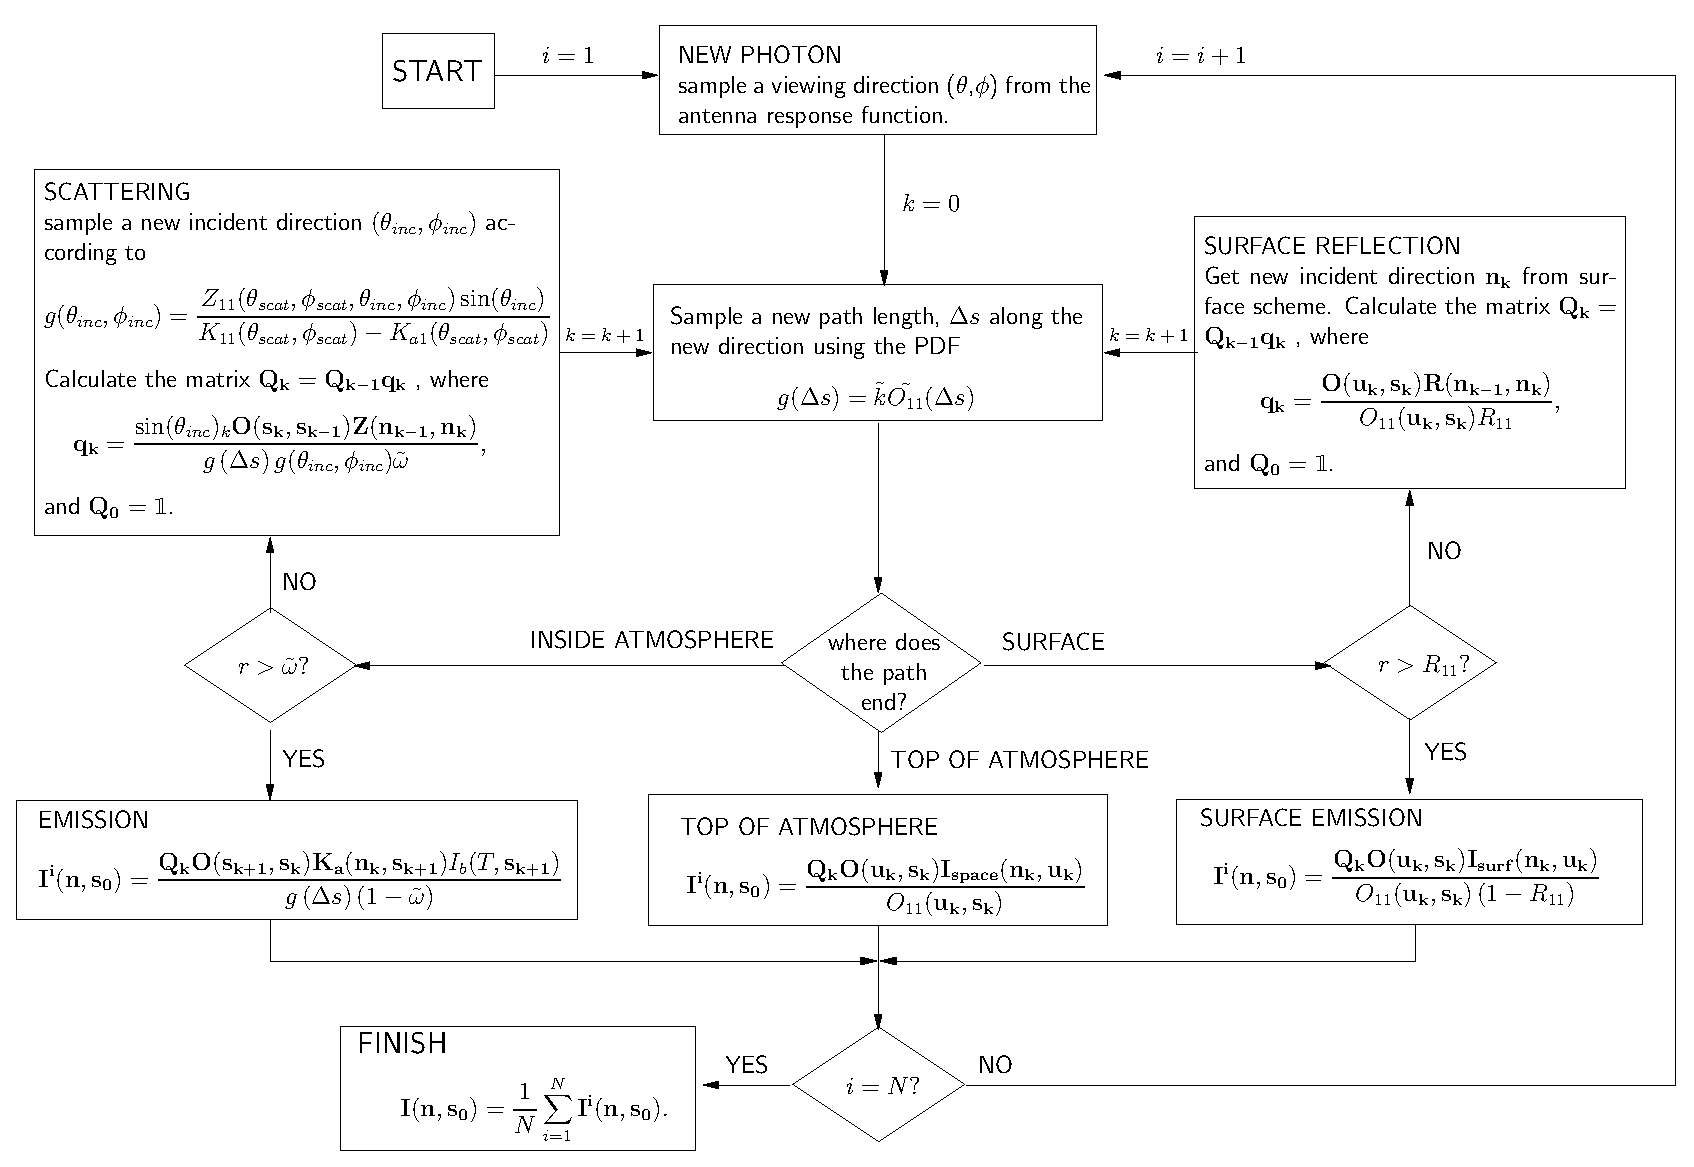
\includegraphics[width=\vsize,angle=90]{flowchart2}
\caption{Flowchart illustrating MCGeneral algorithm}
\end{center}
\label{fig:montecarlo:flowchart}
\end{figure}

\section{Practical considerations regarding optical properties}
\subsection{Particle orientation and the evolution operator}
The calculation of the evolution operator in Eqs. \ref{OconstK} and  \ref{Ogeneral} requires evaluation of the matrix exponential.  If the scattering particles are spheres (P10), or randomly orientated (p20), as described in Section [{\bf FIXME}], then Eq. \ref{OconstK} is simply
\begin{equation}
O_{jj}(s',s)=\exp\left(-K_{jj}\Delta s\right)
\label{OconstKp1020}
\end{equation}
If scattering particles have rotational symmetry, and the axis of symmetry is oriented vertically, or if the particles are have random azimuthal orientation (p30), as described in Section [{\bf FIXME}], then the extinction matrix has a 
block diagonal form with 3 independent elements, $K_{jj}$, $K_{12}$, and $K_{34}$ (See section [{\bf FIXME}]).

\subsection{Particle orientation and the phase matrix}
\section{Variations on the ARTS-MC algorithm}
\subsection{The original ARTS-MC and forcing the original pathlength sample to be within the 3D box} 
\subsection{1D clear sky variables and clear sky radiance look up} 
\subsection{MCIPA}
\subsection{optical path and ice water path calculations}

%%% Local Variables: 
%%% mode: latex 
%%% TeX-master: "uguide" 
%%% End:

